\documentclass[a4paper]
{article}

%Configurações de Idioma e Entrada
\usepackage[utf8x]{inputenc}
\usepackage[brazil]{babel}
\usepackage{ae}
\usepackage{indentfirst}

%Tabelas coloridas com HTML
\usepackage[table,xcdraw]{xcolor}

%Símbolos matemáticos
\usepackage{amsmath,amssymb}
\usepackage{wasysym}

%Inserção de bibliografia
\usepackage{natbib}
%\usepackage[alf]{abntcite}
\renewcommand{\bibname}{Bibliografia}

%Inserção de Figuras e URLs no texto
\usepackage{graphicx,url}


\title{Plano de Trabalho}


\date{January 2021}

\newcommand{\TITULO}{Pré-processamento de imagens hiper-espectrais}
\newcommand{\Autor}{Gabriel Ayres de Oliveira}
\newcommand{\Orientador}{Luís Geraldo Pedroso Meloni, D.Sc.}

\newcommand{\Dia}{06 }
\newcommand{\Mes}{Dezembro }
\newcommand{\Ano}{2021}

\begin{document}


\thispagestyle{empty}
\begin{center}

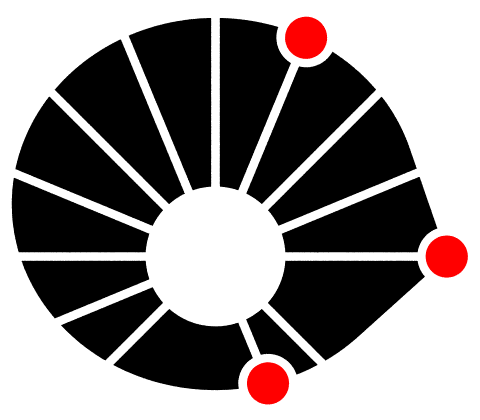
\includegraphics[width=3.0cm]{logo-unicamp.png}\\
\medskip
Universidade Estadual de Campinas\\
Faculdade de Engenharia Elétrica\\


\vfill

{Plano de Trabalho} \\

\vfill


\textbf{\MakeUppercase{\TITULO}}\\

\vfill


\Autor\\

Orientador: \Orientador

\vfill

Campinas\\
\Ano\\

\end{center}
\newpage

\newpage

\tableofcontents
\newpage
\section{Introdução}

Lorem ipsum

\newpage
\section{Proposta e Objetivos}

Lorem ipsum dolor 
\newpage
\section{Conclusão}

Lorem ipsum dolor sit amet

\newpage
\bibliographystyle{unsrt}
\bibliography{references}
\end{document}



